\documentclass[letterpaper]{article}
\usepackage{graphicx} % Required for inserting images
\usepackage{authblk}
%configure print geometry
\usepackage[margin=1.2in]{geometry}
\setlength{\parskip}{0.3\baselineskip}
% preferred reference package
\usepackage[style=numeric, sorting=none]{biblatex}
\addbibresource{refs.bib}

\title{Classic Game Glitches as Cybersecurity Case Studies}
\author[1]{Jon Craton}
\affil[1]{Anderson University, Anderson, IN}
\date{} % no date, we will add it to the final version in the header

\begin{document}

\maketitle

\begin{abstract}
A proposal is presented to use classic videogame glitches as case studies to demonstrate key concepts in computer science and cybersecurity. Two example cases are provided and explored. One case is evaluated as a learning instrument based on its use in an undergraduate computer science classroom.
\end{abstract}

\section{Introduction}
One challenging aspect of teaching is presenting material in a manner that is both authentic and engaging. While it would be nice if we could all arrive to a learning experience prepared to learn for the sake of learning, this is not always the case. While it is certainly possible to coerce students into educational activities via grades or the threat of a quiz or exam, it is beneficial to find ways to encourage intrinsic motivation \cite{deci2013intrinsic}.

In order for teaching to be engaging for students, it is important for it to be genuinely exciting for the teacher. As Parker Palmer notes, "As I teach I project the condition of my soul onto my students, my subject, and our way of being together." \cite{palmer2000courage}. Finding ways to add real exploration and excitement to teaching is valuable both for both teachers and learners.

It can be intimidating for educators to include live demonstrations in their teaching, especially if these demonstrations require skill and can fail in various ways for technical reasons. A lecture has very few failure modes, whereas more complex learning experiences can run into various challenges. There is real benefit to taking this risk, though , as Ken Bain identifies: "The best teaching isoften both an intellectual creation and a performing art. It is both Rembrandt’s brush strokes and the genius of insight, perspective, originality, comprehension, and empathy that makes a Dutch Master." \cite{bain2004best}.

Part of good teaching is creating learning experiences that allow students to become open to a state where the deepest forms of knowledge acquisition can occur. It is not enough for studnets to listen and take notes, they must at times be truly confused and confront their ignorance with humility. This state has been described by Csikszentmihalyi in various ways including  "what a painter feels when the colors on the canvas begin to set up a magnetic tension with each other, and a new thing, a living form, takes shape in front of the astonished creator" \cite{csikszentmihalyi1990flow}.

Students are not merely learning static concepts that can be conveyed as facts from one person to another. Situated learning reminds us that a concept "will continually evolve with each new occasion of use, because new situations, negotiations, and activities inevitably recast it in a new, more densely textured form" \cite{brown1989situated}.

Kolb identified that true learning happens when we encounter a new experience, reflect on it, develop an abstract conceptualization, and engage in active experimentation \cite{kolb84}. Glitches in classic games provide an ideal platform to craft this learning cycle. An initial exploration brings with it a moment of confusion as assumptions about the simulated world are violated. This is followed by additonal observation of the world that allows learners to construct a more accurate model of what is really happening behind the scenes. Finally, learners can test assumptions about their understanding via further experimentation in the world.

As educators, it can be tempting to lean heavily on direct instuction. It allows for a relatively simple planning and execution while making a teacher out of anyone who can read text off of a slide deck. However, a large body of research demonstrates that this approach is not best for learners. Active learning enhances student performance in STEM fields \cite{freeman2014active} and helps to close achievement gaps for underrepresented students \cite{theobald2020active}.

Case studies are a common tool in education. They allow students to explore and apply concepts to real-world situations. They have been shown to be valuable in computer science education as they may be better able to capture the multi-dimensional decisions necessary to construct a correct and effective computer program \cite{linn1992case}.

Videogame glitches are engaging to some learning by their nature. It has been noted that some people play videogames enjoy videogame glitches: "one of the many ways in which a player may enjoy a video game is to explore it in search of these discrepancies, relishing the variety of effects they can cause" \cite{bainbridge2007creative}.

\section{Methods}
An exploration of an in-game glitch first requires a mechanism that allows the glitch to be demonstrated and explored live in a classroom setting. This can be done by connecting a classic console to the classroom projection system, but this creates a number of challenges. It is tedious to transport and connect the system, but it also has limited ability to inspect and debug running games. For this reason, it is often best to use some form of emulation. For this exploration, the open source higan emulator was used \cite{ginder2004higan}.

In order to run a game under emulation, it is necessary to create an image of the read-only memory found on a game cartridge. There are various hardware tools and methods to accomplish this. Once the ROM file has been copied it can be stored for later use. Specialized hardware is not required during emulation.

The case proposed in this paper involves a well-known glitch colloquially referred to as the "Old man glitch". It is well understood and its underlying mechanics have already been described \cite{bulbapedia2005} \cite{scrumpy2016missing}.

This glitch induces the system to access and use memory that has not been properly initialized. In particular, it requires the player character in the game to engage in a wild Pokemon battle when the wild Pokemon data is not properly initialized. This allows the player to encounter and capture invalid or "glitch" Pokemon as shown below:

\noindent % Prevents indentation
\begin{minipage}{\textwidth}
    \centering
    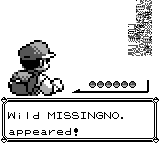
\includegraphics[width=0.4\textwidth]{missingno.png}
    \label{fig:missingno}
\end{minipage}

From a cybersecurity standpoint, it can be valuable to consider the root cause of this issue. Perhaps it could be mapped to an appropriate framework, such as identifying the cause as "Use of Uninitialized Resources" (CWE-908) \cite{mitre2012}.

\section{Findings}
Students were pre-tested prior to the learning experience and post tested afterwards. Quantitatively, a paired-samples t-test indicated a statistically significant increase in scores from the pre-test (M=70.37,SD=30.93) to the post-test (M=92.59,SD=14.70), with a p-value of p=0.0497.

\subsection{First Interesting Finding}
Cum ex unum perpetua, nobis minimum fastidii cu eos. Consul eirmod maiestatis an mei, pro in unum accusata expetendis. Ad vix ceteros eloquentiam, quidam nonumes constituto eos ei. Iudico percipitur eu pri, per eros falli elitr ex. Et eam equidem eleifend, accusam accusamus no his. Mei id tollit prompta qualisque, eu paulo audiam vivendo has, vim ad nemore luptatum voluptaria.

\subsection{Second Interesting Finding}
Movet iriure maluisset et cum, nam tamquam ocurreret voluptatibus cu, an mea idque prompta eligendi. Cum ne dolore nullam singulis, in meliore epicuri forensibus vim. Sed feugait quaestio voluptatum ea. Eirmod omnium civibus ad mei, te sit malorum euismod disputationi. Vitae iisque quo no, ut mea sint appetere euripidis.

\section{Discussion}
Quo nullam eripuit reformidans ad, ex ius mutat eligendi, ex vel duis urbanitas prodesset. No placerat qualisque disputando nam. Idque aliquip cotidieque no his, ea duo homero percipitur, nemore vocibus torquatos no mei. Antiopam complectitur pro ex, stet case theophrastus at his, vel ex amet salutandi constituto.

Mazim percipitur pro et, quas aperiri luptatum eos no. Habeo feugiat meliore mel te. Duo dico ludus epicurei id, sanctus perfecto periculis eu mel. Ad sed dolorum feugait, qui quaeque fabulas ei, appareat intellegebat ut eam.

In vel modus putent scribentur. Prima aliquip definiebas sea ex, modus delicata vituperata ne vix, et mel eius mundi legendos. Ne eos affert inimicus, at mel causae incorrupte. Pro ad soluta aliquid senserit, eu eum noster appetere invidunt. Vocent senserit hendrerit cum ex, adipisci antiopam per ea.

Te essent vivendo moderatius usu. Zril delicata mediocritatem cum in, diceret eleifend mea ex. Mundi graeco periculis quo ut, ei eum libris ullamcorper. Duo fastidii theophrastus id. Vix nostrud intellegam an, usu in tibique interpretaris. Sea possit fuisset an, eum altera vidisse platonem in.

\section{Conclusion}
Vis id verterem expetendis. Vix eros graeci constituto ex. Ullum aeque accommodare mea id, ex euismod ullamcorper eum. Usu probo adipisci id, ut eos tractatos comprehensam. Summo partiendo per ad, ad vix ceteros evertitur. Mel elitr corrumpit definiebas ne.

%\bibliographystyle{plain}
%\bibliography{refs}

\printbibliography
\end{document}
